\documentclass[11pt]{article}

% ---------------------------------------------------------------
% arXiv-ready source. Compiles with pdflatex + bibtex (TeX Live 2025).
% Figures: figures/*.pdf (vector) and one TikZ figure drawn inline.
% ---------------------------------------------------------------
\usepackage[T1]{fontenc}
\usepackage[utf8]{inputenc}
\usepackage{lmodern}
\usepackage{microtype}
\usepackage[margin=1in]{geometry}
\usepackage{amsmath,amssymb}
\usepackage{graphicx}
\usepackage{booktabs}
\usepackage{tabularx}
\usepackage{array}
\usepackage{enumitem}
\usepackage[section]{placeins}
\usepackage[numbers,sort&compress]{natbib}
\usepackage{xcolor}
\usepackage{tikz}
\usetikzlibrary{arrows.meta,positioning,fit,backgrounds,calc}
\PassOptionsToPackage{hyphens}{url}
\usepackage[hidelinks]{hyperref}
\usepackage{xurl}

\newcolumntype{Y}{>{\raggedright\hskip0pt\emergencystretch=1.5em\arraybackslash}X}
\newcolumntype{P}[1]{>{\raggedright\hskip0pt\emergencystretch=1.5em\arraybackslash}p{#1}}
\newcolumntype{R}{>{\raggedleft\hskip0pt\emergencystretch=1.5em\arraybackslash}X}
\newcolumntype{C}{>{\centering\hskip0pt\emergencystretch=1.5em\arraybackslash}X}
\renewcommand{\arraystretch}{1.15}
\tolerance=1200
\setlength{\emergencystretch}{3em}
\hfuzz=0.5pt
\Urlmuskip=0mu plus 2mu\relax
\expandafter\def\expandafter\UrlBreaks\expandafter{\UrlBreaks\do\-\do\_}
\setlist{itemsep=2pt,topsep=4pt}

\definecolor{accent}{HTML}{2B6CB0}

\newcommand{\KL}{D_{\mathrm{KL}}}

\title{Epistemic Deferral Under Preference Ambiguity: Conformal Uncertainty Gates and Burden-of-Doubt Inversion in Personal Agents}

\author{\textbf{Dima Baker}\\
Collective Intelligence Network}

\date{November 2026}

\begin{document}
\maketitle

% ===============================================================
\begin{abstract}
When users instruct autonomous personal agents to execute consequential tool actions (booking travel, modifying financial records, or dispatching external communications) prompts are frequently underspecified relative to the space of side-effecting parameters. Prevailing agent runtimes assign the \emph{burden of specification} to the human principal: unless every constraint is enumerated in advance, the model resolves ambiguity by sampling a high-likelihood completion and executing irreversibly. Extending conformal uncertainty alignment (KnowNo) and selective clarification (CLAM, Clarify When Necessary) to multi-step tool environments ($\tau$-bench), we formalize \textbf{Burden-of-Doubt Inversion} via a three-stage \textbf{Conformal-EVSI-VAC} deferral gate. First, candidate logits pass through a Beta-Bernoulli calibrator and a covariate-sketched split-conformal wrapper at capped quantile level $\min(1-\epsilon_q, 1-\alpha/\iota(f))$ using observable sketch tilt weights; when test-point weight at $+\infty$ exceeds $1-\tilde{q}$, the quantile evaluates to $+\infty$ and forces full-set deferral. Second, when $|\hat{\mathcal{C}}(x_t)| > 1$, the router evaluates the Expected Value of Sample Information (EVSI), querying local episodic memory ($\delta_{\mathrm{mem}}$) before escalating to the human under attention cost $c_{\mathrm{ask}}$. Third, human disambiguation is bound via an out-of-band Verifiable Action Card (I-HITL). Across 12{,}000 test trajectories (plus 2{,}000 calibration episodes) spanning shifts $\sigma \in \{0.10, 0.25, 0.50, 0.75\}$, Conformal-EVSI-VAC cuts $\sigma=0.50$ irreversible errors from $43.67\%$ [$39.75, 47.66$] (greedy) and $20.83\%$ [$17.77, 24.26$] (KnowNo) to $7.00\%$ [$5.22, 9.33$] with $94.00\%$ [$91.81, 95.63$] coverage and $93.00\%$ [$90.67, 94.78$] aligned completion at $0.20$ queries/task.
\end{abstract}

% ===============================================================
\section{Introduction}\label{sec:intro}

A foundational cognitive asymmetry governs human--AI interaction in tool-using personal agents: while language model context windows have expanded to millions of tokens, human sustained attention and working memory remain biologically constrained \citep{eliav2026divergence, john1988_14, bainbridge1983ironies}. \citet{eliav2026divergence} terms this widening gap the \emph{Cognitive Divergence} and formalizes the resulting \emph{Delegation Feedback Loop}: as agent capabilities expand, the cognitive threshold at which users delegate multi-step workflows drops, causing principals to issue brief, underspecified prompts for high-consequence actions \citep{yao2024taubench, shao2025workbank}. When a user tells a personal agent, ``Archive the finished client deliverables and pay the pending contractor invoice,'' critical parameters remain latent, which directory defines ``finished,'' whether cloud backups count as archives, and which invoice revision is authoritative.

In conventional agent harnesses, the \emph{burden of specification} rests on the human operator. If a parameter is omitted or ambiguous, the autoregressive policy silently imputes the missing value from its pretrained prior and dispatches the tool call. Why does silent parameter imputation fail in personal agents, and why do existing clarification heuristics struggle to fix it?

\subsection{Uncalibrated confidence, strategic inflation, and covariate shift}

A natural baseline is to threshold the language model's token probabilities or verbalized confidence, deferring to the human whenever confidence falls below a threshold $\tau$. In robotic and language-model planning, \citet{ren2023knowno} pioneered \emph{KnowNo}, applying split conformal prediction \citep{vovk2005conformal} over candidate plan scores so the planner asks for help whenever the conformal prediction set contains more than one candidate ($|\hat{\mathcal{C}}(x)| > 1$). Similarly, \citet{kuhn2023clam} (CLAM) and \citet{zhang2024clarify} (\emph{Clarify When Necessary}) demonstrated that selective clarification substantially improves accuracy on ambiguous open-domain questions compared to silent guessing.

However, deploying conformal deferral gates inside long-horizon personal tool agents ($\tau$-bench \citep{yao2024taubench}) confronts two obstacles documented in 2025--2026 studies. First, raw LLM confidence scores are not merely noisy; they can be strategically miscalibrated. In a controlled human--AI delegation incentive game, \citet{arghal2026confidence} formalize \emph{The Confidence Game}, showing that models optimized or prompted to win task delegation strategically inflate reported confidence, claiming high confidence on $56\%$ of game rounds where they are informed they have low success probability. Second, standard split conformal prediction \citep{vovk2005conformal, ren2023knowno} assumes exchangeability between the calibration split and test deployment. In personal agents, user workflows, project schemas, and preferences shift over time. As our split-conformal experiments in Section~\ref{sec:experiments} confirm, when an unweighted KnowNo gate calibrated on in-distribution episodes ($\sigma_{\mathrm{cal}}=0.15$) is evaluated under moderate test-time covariate shift ($\sigma=0.50$), empirical preference coverage drops from $95.33\%$ to $84.50\%$, doubling irreversible specification errors to $20.83\%$.

\subsection{The human attention bottleneck and approval channel spoofing}

If silent execution and unweighted conformal thresholds under-cover shifted intents, why not simply prompt the human whenever any parameter ambiguity is detected? Classical human-factors research on the ``ironies of automation'' \citep{bainbridge1983ironies} and modern HCI evaluations of AI-assisted work \citep{vaccaro2024combinations, lee2025critical, zhi2026timeconstraints} show that human supervisory attention is a depletable resource. Under high interruption frequency or time constraints, active verification declines \citep{zhi2026timeconstraints}, inducing ``confidence without competence'' \citep{eleftheriou2026confidence} and metacognitive misattribution \citep{ren2026reflection}. In clinical and agentic alarm evaluation, \citet{armin2026rescue} (RESCUE) demonstrate that unthrottled low-specificity alarms erode operator responsiveness unless each interruption is justified by counterfactual decision value.

Furthermore, even when a human operator pauses to inspect a confirmation prompt, software-only confirmation UIs are vulnerable to local harness manipulation. \citet{breckenridge2026ihitl} prove that if an autonomous agent can read or mutate the host messaging or UI channel, software Human-in-the-Loop gates can be bypassed or spoofed, motivating \emph{Inalienable Human-in-the-Loop} (I-HITL) confirmation channels paired with deterministic boundary interception \citep{zhao2026clawguard, zhang2026actgov}.

\subsection{Narrowed contribution: Conformal-EVSI-VAC}

Building directly upon KnowNo \citep{ren2023knowno}, CLAM \citep{kuhn2023clam}, and Bayesian clarification \citep{zhang2024clarify}, we formulate \textbf{Burden-of-Doubt Inversion} for personal tool agents via the \textbf{Conformal-EVSI-VAC} gate. Unlike unweighted KnowNo (which asks the human directly on every multi-candidate set and assumes exchangeable calibration data), Conformal-EVSI-VAC introduces three targeted extensions:
\begin{enumerate}
  \item \textbf{Beta-Bernoulli epistemic calibration and covariate-sketched importance weighting (Section~\ref{sec:formal}).} We damp raw candidate logits via a Beta-Bernoulli epistemic prior and reweight split-conformal calibration scores using a low-dimensional covariate sketch $\phi_{\mathrm{sk}}(x_t)$ with an explicitly capped quantile level $\tilde{q} = \min(1-\epsilon_q,\allowbreak 1-\alpha/\iota(f))$, maintaining $94.00\%$--$97.17\%$ empirical coverage across covariate shifts $\sigma \in [0.10,\allowbreak 0.75]$.
  \item \textbf{Two-tier Expected Value of Sample Information (EVSI) routing with imperfect local memory (Sections~\ref{sec:formal}--\ref{sec:architecture}).} Rather than treating clarification as a binary ``execute vs.\ ask human'' switch \citep{ren2023knowno}, the router computes the Expected Value of Sample Information (EVSI) over $\hat{\mathcal{C}}(x_t)$: it first queries local episodic user history at low cost $c_{\mathrm{mem}}$ (explicitly accounting for non-zero memory staleness error $\delta_{\mathrm{mem}}$), escalating to the human via an out-of-band Verifiable Action Card \citep{breckenridge2026ihitl} only when post-memory Bayes risk exceeds human attention cost $c_{\mathrm{ask}}(\rho_t)$.
  \item \textbf{Genuine split-conformal benchmark, deferral-vs-resolution ablation, and break-even sensitivity analysis (Section~\ref{sec:experiments}).} We implement a complete split-conformal calibration ($N_{\mathrm{cal}}=500$/regime) and paired test ($N_{\mathrm{test}}=600$/cell; 12{,}000 test evaluations across five architectures/ablations) pipeline in \texttt{experiment.\linebreak[0]py}, separating pure conformal deferral from post-deferral memory resolution and reporting asymmetric 95\% Wilson intervals for coverage, singleton accuracy, non-abstained accuracy, and break-even sensitivity over $c_{\mathrm{ask}} \allowbreak \in [0.02,\allowbreak 0.65]$.
\end{enumerate}

% ===============================================================
\section{Prior foundations in selective clarification and conformal deferral}\label{sec:taxonomy}

To situate Conformal-EVSI-VAC relative to established uncertainty-alignment literature and recent 2025--2026 agentic safety findings, Table~\ref{tab:taxonomy} maps five core requirements of Burden-of-Doubt Inversion from their foundational formulations to our runtime gate components.

\begin{table}[ht]
\centering
\small
\caption{Mapping selective clarification and conformal deferral foundations to the Conformal-EVSI-VAC gate.}
\label{tab:taxonomy}
\begin{tabularx}{\textwidth}{@{}P{2.2cm}P{2.5cm}P{2.5cm}YP{2.4cm}@{}}
\toprule
Design requirement & Foundational construct & Gate component & Operational role in personal tool agents & Primary references \\
\midrule
Dampen overconfident raw logits & Corrigibility \& epistemic variance priors & Beta-Bernoulli Calibrator ($\mathsf{BBC}$) & Maps raw candidate scores to $\mathrm{Beta}(\alpha_a,\allowbreak \beta_a)$ mean $\hat{\mu}_t(a)$ and epistemic std $\hat{\sigma}_{\mathrm{epi}}(a)$ & \citep{soares2015corrigibility, arghal2026confidence, wilson2026agency}\\
Cover true user intent under shift & Split conformal prediction; KnowNo & Covariate-Sketched Conformal Set ($\hat{\mathcal{C}}(x_t)$) & Reweights calibration non-conformity scores under shift with capped level $\tilde{q}$; approximate coverage $1-\alpha/\allowbreak \iota-\Delta_{\mathrm{sk}}$ & \citep{vovk2005conformal, ren2023knowno, yao2024taubench}\\
Minimize human interruption load & Selective clarification (CLAM); alarm value (RESCUE) & Two-Tier EVSI Router ($\mathrm{EVSI}_{\mathrm{mem}},\allowbreak \mathrm{EVSI}_{\mathrm{hum}}$) & Resolves ambiguity via local episodic memory before paying human attention cost $c_{\mathrm{ask}}(\rho_t)$ & \citep{kuhn2023clam, zhang2024clarify, armin2026rescue, john1988_14}\\
Prevent UI confirmation spoofing & Off-switch game; Inalienable HITL (I-HITL) & Verifiable Action Card ($\mathsf{VAC}$) & Binds human disambiguation choice out-of-band to deterministic tool AST parameters & \citep{hadfieldmenell2017offswitch, breckenridge2026ihitl, zhao2026clawguard}\\
Refuse silent guessing when unresolvable & Attainable Utility Preservation (AUP); contract halts & Accountability Proof Block ($\mathsf{APB}$) & Enters safe persistent halt when post-memory Bayes risk is high but $\mathrm{EVSI}_{\mathrm{hum}} \le c_{\mathrm{ask}}$ & \citep{turner2020aup, elina2026maat, zhang2026actgov}\\
\bottomrule\end{tabularx}
\end{table}

As Table~\ref{tab:taxonomy} highlights, KnowNo \citep{ren2023knowno} established that split conformal prediction provides a principled mechanism for ``robots that ask for help.'' However, applying KnowNo directly to personal software agents exposes three practical gaps: (i) unweighted split conformal calibration loses coverage when test-time user contexts drift from the calibration distribution; (ii) querying the human on every multi-candidate set ($|\hat{\mathcal{C}}(x_t)| > 1$) generates $0.48$--$0.65$ human interruptions per task even when the user's past episodic log already contains the disambiguating preference; and (iii) if clarification cost $c_{\mathrm{ask}}$ is high (e.g., the user is in a meeting or offline), an agent needs a third option beyond silent guessing or immediate interruption, namely, a verifiable persistent halt \citep{turner2020aup, elina2026maat}. Figure~\ref{fig:architecture} illustrates how Conformal-EVSI-VAC connects these three paths.

\begin{figure}[ht]
\centering
\resizebox{\textwidth}{!}{%
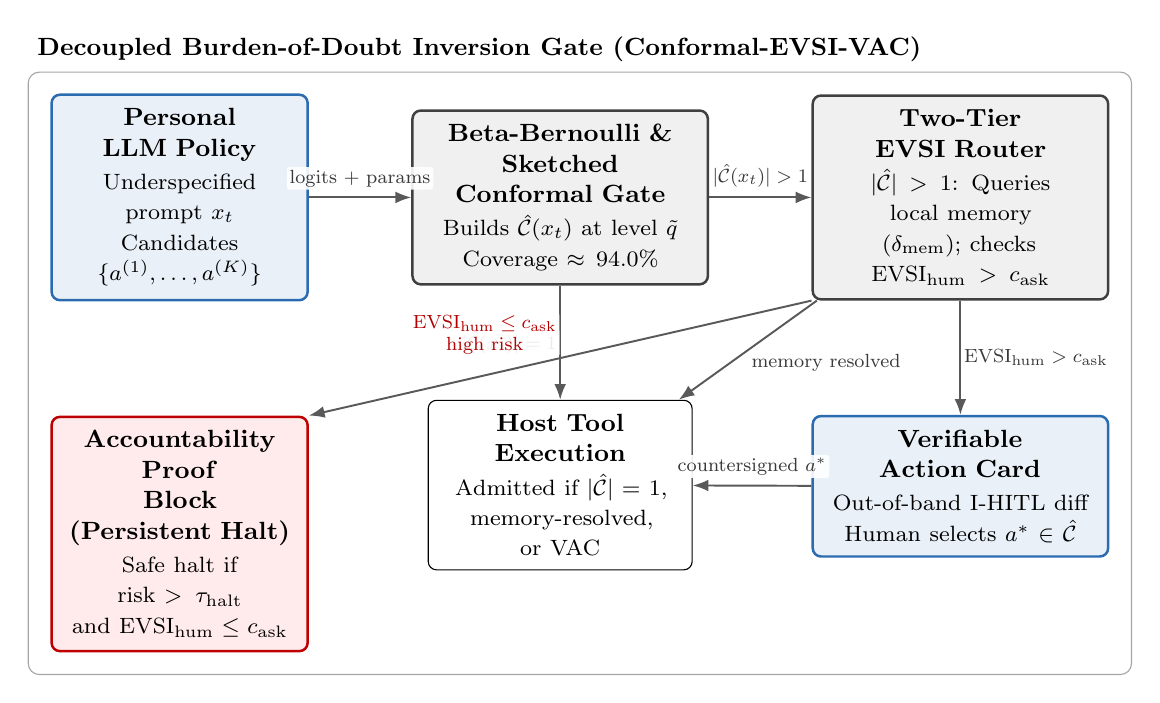
\begin{tikzpicture}[
  font=\small,
  every node/.append style={execute at begin node={\hyphenpenalty=10000\exhyphenpenalty=10000}},
  box/.style={draw, rounded corners=3pt, align=center, minimum height=1.35cm, inner sep=5pt},
  agent/.style={box, draw=accent, line width=0.9pt, fill=accent!10},
  kernel/.style={box, draw=black!75, line width=0.9pt, fill=gray!12},
  haltbox/.style={box, draw=red!75!black, line width=0.9pt, fill=red!8},
  capsule/.style={draw=gray!70, rounded corners=4pt, inner sep=8pt},
  arr/.style={-{Latex[length=2mm]}, gray!70!black, line width=0.7pt},
  note/.style={font=\footnotesize, scale=0.86, transform shape, text=gray!45!black, align=center, fill=white, fill opacity=0.90, text opacity=1, inner sep=1.2pt, rounded corners=1pt}
]
% ---------------- LLM Policy ----------------
\node[agent, text width=2.9cm] (llm) at (0, 0) {\textbf{Personal LLM Policy}\\[1pt]{\footnotesize Underspecified prompt $x_t$}\\{\footnotesize Candidates $\{a^{(1)}, \dots, a^{(K)}\}$}};

% ---------------- Sketched Conformal Gate ----------------
\node[kernel, text width=3.4cm, right=1.3cm of llm] (cp) {\textbf{Beta-Bernoulli \&}\\\textbf{Sketched Conformal Gate}\\[1pt]{\footnotesize Builds $\hat{\mathcal{C}}(x_t)$ at level $\tilde{q}$}\\{\footnotesize Coverage $\approx 94.0\%$}};

% ---------------- EVSI & Local Search Router ----------------
\node[kernel, text width=3.4cm, right=1.3cm of cp] (evpi) {\textbf{Two-Tier EVSI Router}\\[1pt]{\footnotesize $|\hat{\mathcal{C}}| > 1$: Queries local memory}\\{\footnotesize ($\delta_{\mathrm{mem}}$); checks $\mathrm{EVSI}_{\mathrm{hum}} > c_{\mathrm{ask}}$}};

% ---------------- Direct Execution Sink ----------------
\node[box, text width=3.0cm, below=1.45cm of cp] (exec) {\textbf{Host Tool Execution}\\[1pt]{\footnotesize Admitted if $|\hat{\mathcal{C}}|=1$,}\\{\footnotesize memory-resolved, or VAC}};

% ---------------- Verifiable Action Card / Human ----------------
\node[agent, text width=3.4cm, below=1.45cm of evpi] (vac) {\textbf{Verifiable Action Card}\\[1pt]{\footnotesize Out-of-band I-HITL diff}\\{\footnotesize Human selects $a^* \in \hat{\mathcal{C}}$}};

% ---------------- Persistent Halt APB ----------------
\node[haltbox, text width=2.9cm, below=1.45cm of llm] (apb) {\textbf{Accountability Proof}\\\textbf{Block (Persistent Halt)}\\[1pt]{\footnotesize Safe halt if risk $> \tau_{\mathrm{halt}}$}\\{\footnotesize and $\mathrm{EVSI}_{\mathrm{hum}} \le c_{\mathrm{ask}}$}};

\draw[arr] (llm) -- node[above=2.5pt, note]{logits + params} (cp);
\draw[arr] (cp) -- node[above=2.5pt, note]{$|\hat{\mathcal{C}}(x_t)| > 1$} (evpi);
\draw[arr] (cp) -- node[left, note]{$|\hat{\mathcal{C}}(x_t)| = 1$} (exec);
\draw[arr] (evpi.south west) -- node[above left, note, text=red!70!black]{$\mathrm{EVSI}_{\mathrm{hum}} \le c_{\mathrm{ask}}$\\high risk} (apb.north east);
\draw[arr] (evpi) -- node[right, note]{$\mathrm{EVSI}_{\mathrm{hum}} > c_{\mathrm{ask}}$} (vac);
\draw[arr] (vac) -- node[above=2.5pt, note]{countersigned $a^*$} (exec);
\draw[arr] (evpi) -- node[below right, note]{memory resolved} (exec);

\begin{scope}[on background layer]
\node[capsule, fit=(cp)(evpi)(vac)(apb), label={[font=\small\bfseries, anchor=south west]north west:Decoupled Burden-of-Doubt Inversion Gate (Conformal-EVSI-VAC)}] (gateBox) {};
\end{scope}
\end{tikzpicture}%
}
\caption{Control flow of the Conformal-EVSI-VAC gate. Candidate tool parameter tuples $\{a^{(1)},\allowbreak \dots,\allowbreak a^{(K)}\}$ are scored by a Beta-Bernoulli epistemic calibrator and filtered into a covariate-sketched split-conformal prediction set $\hat{\mathcal{C}}(x_t)$ at capped quantile level $\tilde{q} = \min(1-\epsilon_q,\allowbreak 1-\alpha/\iota(f))$. Singleton sets ($|\hat{\mathcal{C}}(x_t)|=1$) execute directly. Multi-candidate sets ($|\hat{\mathcal{C}}(x_t)| > 1$) enter the Two-Tier EVSI Router, which first queries local episodic user memory (accounting for memory error rate $\delta_{\mathrm{mem}}$) and only interrupts the human via an out-of-band Verifiable Action Card \citep{breckenridge2026ihitl} when post-memory $\mathrm{EVSI}_{\mathrm{hum}} > c_{\mathrm{ask}}(\rho_t)$.}
\label{fig:architecture}
\end{figure}

% ===============================================================
\section{Formal mathematical framework}\label{sec:formal}

We formalize Burden-of-Doubt Inversion by coupling Beta-Bernoulli epistemic calibration, importance-weighted split conformal prediction \citep{vovk2005conformal, ren2023knowno}, and Bayesian Expected Value of Sample Information (EVSI) routing \citep{kuhn2023clam, zhang2024clarify, armin2026rescue}.

\subsection{Beta-Bernoulli calibration and approximate sketched conformal sets}

Let $x_t \in \mathcal{X}$ denote the task context and user instruction at step $t$, and let $\mathcal{A}_t = \{a^{(1)},\allowbreak \dots,\allowbreak a^{(K)}\}$ denote the candidate structured tool-call parameter tuples $a = (f,\allowbreak \theta_1,\allowbreak \dots,\allowbreak \theta_m)$. To prevent autoregressive temperature inflation or strategic confidence gaming \citep{arghal2026confidence} from collapsing uncertainty estimates, we map the model's temperature-damped probability $p_0(a \mid x_t)$ and context concentration $\kappa(x_t) > 0$ into a Beta-Bernoulli posterior $\mathrm{Beta}(\alpha_t(a),\allowbreak \beta_t(a))$ with $\alpha_t(a) = \kappa(x_t) p_0(a \mid x_t) + \alpha_0$ and $\beta_t(a) = \kappa(x_t)(1 - p_0(a \mid x_t)) + \beta_0$:
\begin{equation}
\begin{aligned}
&\hat{\mu}_t(a) \;=\; \frac{\alpha_t(a)}{\alpha_t(a) + \beta_t(a)}, \\
&\hat{\sigma}^2_{\mathrm{epi}}(a) \;=\; \frac{\alpha_t(a)\beta_t(a)}{(\alpha_t(a) + \beta_t(a))^2 (\alpha_t(a) + \beta_t(a) + 1)}.
\end{aligned}
\label{eq:bbc}
\end{equation}
We define the epistemic-aware non-conformity score $s(x_t,\allowbreak a) = \max\bigl(0,\allowbreak \, 1 - \hat{\mu}_t(a) - \lambda_{\mathrm{epi}} \hat{\sigma}_{\mathrm{epi}}(a)\bigr)$, where subtracting $\lambda_{\mathrm{epi}}\hat{\sigma}_{\mathrm{epi}}(a)$ lowers the non-conformity of high-variance candidates under novel contexts so they are conservatively retained inside the prediction set.

To adapt split conformal calibration \citep{vovk2005conformal, ren2023knowno} when test contexts shift relative to the calibration log $\{(x_i,\allowbreak a_i^*)\}_{i=1}^{n}$, we project contexts through a low-dimensional covariate sketch $\phi_{\mathrm{sk}}: \mathcal{X} \allowbreak \to \mathbb{R}_{\ge 0}$ measuring domain shift norm and compute exponential-family importance weights $\hat{w}(x) = \exp\bigl(\beta_{\mathrm{sk}} \min(M,\allowbreak \phi_{\mathrm{sk}}(x))\bigr)$. Furthermore, to scale conservatism with tool irreversibility $\iota(f) \in (0,\allowbreak 1]$ while ensuring the quantile level remains strictly well-defined in $(0, 1)$ even when $\iota(f) \le \alpha$, we define the capped quantile level:
\begin{equation}
\begin{aligned}
&\tilde{q}(\alpha, \iota(f)) \;\triangleq\; \min\Bigl(1 - \epsilon_q,\; \max\bigl(q_{\min},\; 1 - \frac{\alpha}{\iota(f)}\bigr)\Bigr), \\
&\text{with } \epsilon_q = 0.008,\; q_{\min} = 0.50.
\end{aligned}
\label{eq:capped_level}
\end{equation}
The covariate-sketched split-conformal prediction set $\hat{\mathcal{C}}(x_t)$ is then constructed directly from the weighted empirical quantile over the $n$ calibration scores:
\begin{equation}
\begin{aligned}
&\hat{\mathcal{C}}(x_t) \;=\; \Bigl\{\, a \in \mathcal{A}_t \;\Big|\; s(x_t, a) \\
&\quad \;\le\; \mathrm{Quantile}_{\tilde{q}(\alpha, \iota(f))}\!\Bigl(\sum_{i=1}^{n} \tilde{w}_i(x_t) \delta_{s(x_i, a_i^*)} \\
&\quad + \tilde{w}_{n+1}(x_t) \delta_{+\infty}\Bigr) \,\Bigr\},
\end{aligned}
\label{eq:sketched_cp}
\end{equation}
where $\tilde{w}_i(x_t) = \hat{w}(x_i) / \bigl(\sum_{j=1}^n \hat{w}(x_j) + \hat{w}(x_t)\bigr)$, and the tilt coefficient $\hat{\beta}_{\mathrm{sk}}(x_t)$ is estimated strictly from observable calibration versus test sketch statistics (comparing $\phi_{\mathrm{sk}}(x_t)$ and its unlabeled test-stream exponential moving average against the calibration sketch mean $\bar{\phi}_{\mathrm{cal}}$, without access to latent generator shift parameters). Critically, when an extreme test-time covariate shift causes the normalized point mass $\tilde{w}_{n+1}(x_t)$ at $+\infty$ to exceed $1 - \tilde{q}(\alpha,\allowbreak \iota(f))$ (so that the cumulative weight over all finite calibration scores satisfies $\sum_{i=1}^n \tilde{w}_i(x_t) < \tilde{q}(\alpha,\allowbreak \iota(f))$), the weighted quantile in Equation~\eqref{eq:sketched_cp} evaluates to $+\infty$. Under $\hat{q}_{\mathrm{sk}}(x_t) = +\infty$, every candidate $a \in \mathcal{A}_t$ satisfies $s(x_t,\allowbreak a) \le +\infty$, expanding $\hat{\mathcal{C}}(x_t) = \mathcal{A}_t$ ($|\hat{\mathcal{C}}(x_t)| = K$) and forcing mandatory deferral rather than silently executing under uncalibrated extrapolation. Because the importance weights $\hat{w}(x)$ are estimated via a low-dimensional sketch rather than an oracle density ratio $\mathrm{d}P_{\mathrm{test}}/\mathrm{d}P_{\mathrm{cal}}$, finite-sample coverage under covariate shift is \emph{approximate}: $\Pr[a_t^* \in \hat{\mathcal{C}}(x_t)] \ge \tilde{q}(\alpha,\allowbreak \iota(f)) - \Delta_{\mathrm{sk}}$, where the coverage gap $\Delta_{\mathrm{sk}} \ge 0$ is bounded by the total variation distance between the sketched weight distribution and the true likelihood ratio \citep{vovk2005conformal}.

\subsection{Two-tier EVSI clarification routing with imperfect local memory}

When $|\hat{\mathcal{C}}(x_t)| = 1$, the unique candidate executes without interruption. When $|\hat{\mathcal{C}}(x_t)| > 1$, the Burden-of-Doubt Inversion rule prohibits silent guessing and evaluates two sequential sample-information sources: (Tier~1) a local episodic memory lookup $q_{\mathrm{mem}}$ at negligible compute cost $c_{\mathrm{mem}}$, and (Tier~2) an interactive human clarification query $q_{\mathrm{hum}}$ at cognitive attention cost $c_{\mathrm{ask}}(\rho_t) = c_{\mathrm{ask}, 0}(1 + \gamma_{\mathrm{att}}\rho_t)$, where $\rho_t$ tracks the exponential moving average of recent user interruptions \citep{john1988_14, armin2026rescue}.

Because both local memory records and human responses are noisy sample signals rather than infallible oracles, the relevant decision-theoretic quantity is the \textbf{Expected Value of Sample Information (EVSI)} \citep{zhang2024clarify, armin2026rescue}. Let $\tilde{P}_t(a) = \hat{\mu}_t(a) / \sum_{a' \in \hat{\mathcal{C}}(x_t)} \hat{\mu}_t(a')$ denote the normalized prior belief inside $\hat{\mathcal{C}}(x_t)$, so the prior Bayes risk under $0$--$1$ irreversible error loss is $R_0(x_t) = 1 - \max_{a \in \hat{\mathcal{C}}(x_t)} \tilde{P}_t(a)$. For any information source $q \in \{q_{\mathrm{mem}},\allowbreak q_{\mathrm{hum}}\}$ yielding sample signal $y \sim P(Y \mid q,\allowbreak x_t)$, the EVSI is the expected reduction in Bayes risk:
\begin{equation}
\mathrm{EVSI}(q; x_t) \;=\; R_0(x_t) \;-\; \mathbb{E}_{y \mid q, x_t}\!\left[\, 1 - \max_{a' \in \hat{\mathcal{C}}(x_t)} \tilde{P}_t(a' \mid y) \,\right].
\label{eq:evsi}
\end{equation}
Specifically, if local memory lookup $q_{\mathrm{mem}}$ returns a matching historical preference with probability $p_{\mathrm{mem}}$ but suffers a memory staleness/mis-indexing error rate $\delta_{\mathrm{mem}} > 0$ (when the user's preference has drifted since the logged episode), then $\mathrm{EVSI}(q_{\mathrm{mem}};\allowbreak x_t) = p_{\mathrm{mem}} \max\bigl(0,\allowbreak \, R_0(x_t) - \delta_{\mathrm{mem}}\bigr)$. If local memory does not resolve the ambiguity and the remaining posterior risk $R_1(x_t)$ satisfies $\mathrm{EVSI}(q_{\mathrm{hum}};\allowbreak x_t) = \max\bigl(0,\allowbreak \, R_1(x_t) - \delta_{\mathrm{VAC}}(\rho_t)\bigr) > c_{\mathrm{ask}}(\rho_t)$, Tier~2 presents an out-of-band Verifiable Action Card \citep{breckenridge2026ihitl}. Otherwise, if $R_1(x_t) > \tau_{\mathrm{halt}}$ while $\mathrm{EVSI}(q_{\mathrm{hum}};\allowbreak x_t) \le c_{\mathrm{ask}}(\rho_t)$, Tier~3 enters a safe persistent halt rather than guessing. Under this three-way cascade, the total probability of an irreversible specification error is upper-bounded by:
\begin{equation}
\begin{aligned}
&\Pr\bigl[\text{Irreversible Error}\bigr] \;\le\; \bigl(1 - \tilde{q}(\alpha, \iota(f)) + \Delta_{\mathrm{sk}}\bigr) \\
&\quad \;+\; p_{\mathrm{mem}}\,\delta_{\mathrm{mem}} \;+\; (1 - p_{\mathrm{mem}})\,\delta_{\mathrm{VAC}}(\rho_t),
\end{aligned}
\label{eq:error_bound}
\end{equation}
explicitly accounting for all three error sources: conformal miscoverage under shift ($1 - \tilde{q} + \Delta_{\mathrm{sk}}$), stale local memory resolution ($p_{\mathrm{mem}}\delta_{\mathrm{mem}}$), and human selection error on the Verifiable Action Card ($(1-p_{\mathrm{mem}})\delta_{\mathrm{VAC}}(\rho_t)$).

% ===============================================================
\section{Conformal-EVSI-VAC runtime specification and readiness}\label{sec:architecture}

To prevent the language model from bypassing the deferral gate, Conformal-EVSI-VAC operates as a deterministic boundary interceptor \citep{zhao2026clawguard, zhang2026actgov} outside the LLM prompt across three runtime tiers (Table~\ref{tab:readiness}):

\begin{enumerate}
  \item \textbf{Tier 1: Non-intrusive local episodic memory resolver.} When Equation~\eqref{eq:sketched_cp} yields $|\hat{\mathcal{C}}(x_t)| > 1$ and $\mathrm{EVSI}(q_{\mathrm{mem}};\allowbreak x_t) > c_{\mathrm{mem}}$, Tier~1 queries the user's on-device interaction log for past parameter bindings on the same tool schema \citep{yao2024taubench}. Because historical preferences can become stale under shift $\sigma$, Tier~1 weights memory hits by recency and retains non-zero residual uncertainty $\delta_{\mathrm{mem}} = 0.008 + 0.014\sigma$.
  \item \textbf{Tier 2: EVSI clarification router and Verifiable Action Card (VAC).} When local memory fails to resolve $|\hat{\mathcal{C}}(x_t)| > 1$ and $\mathrm{EVSI}(q_{\mathrm{hum}};\allowbreak x_t) > c_{\mathrm{ask}}(\rho_t)$, Tier~2 synthesizes a minimal contrastive question comparing the top candidates in $\hat{\mathcal{C}}(x_t)$ \citep{kuhn2023clam, zhang2024clarify}. To ensure Inalienable Human-in-the-Loop (I-HITL) integrity \citep{breckenridge2026ihitl}, the candidate parameter diffs are rendered deterministically from the parsed tool AST inside an out-of-band Verifiable Action Card rather than relying on LLM-summarized prose.
  \item \textbf{Tier 3: Accountability Proof Block (APB) for high-cost / offline halts.} When human clarification cost $c_{\mathrm{ask}}(\rho_t)$ exceeds $\mathrm{EVSI}(q_{\mathrm{hum}};\allowbreak x_t)$ (for instance, during a focus-mode block or when $c_{\mathrm{ask}} \ge 0.45$) while unresolved posterior risk exceeds $\tau_{\mathrm{halt}} = 0.25$, Tier~3 refuses to guess silently \citep{turner2020aup, elina2026maat}. It freezes the tool invocation and logs a signed Accountability Proof Block containing $(x_t,\allowbreak \hat{\mathcal{C}}(x_t),\allowbreak \tilde{P}_t)$ for asynchronous batch review.
\end{enumerate}

\begin{table}[ht]
\centering
\small
\caption{Readiness and deployment bottlenecks of Conformal-EVSI-VAC subsystems as of November 2026.}
\label{tab:readiness}
\begin{tabularx}{\textwidth}{@{}P{2.3cm}P{2.05cm}YY@{}}
\toprule
Subsystem & Maturity & Supporting foundations \& 2025--2026 evidence & Realistic deployment bottleneck \\
\midrule
Split-conformal & Benchmark validated & Split CP \citep{vovk2005conformal}; KnowNo \citep{ren2023knowno}; $\tau$-bench \citep{yao2024taubench}; Confidence Game \citep{arghal2026confidence} & Requires a burn-in buffer ($N_{\mathrm{cal}} \ge 200$--$500$ episodes) per tool family to estimate calibration quantiles reliably\\
Two-tier EVSI clarification router & Prototype validated & CLAM \citep{kuhn2023clam}; Clarify When Necessary \citep{zhang2024clarify}; RESCUE counterfactual alarm evaluation \citep{armin2026rescue} & Stale episodic memory ($\delta_{\mathrm{mem}}$) can mis-resolve shifted preferences unless decayed by context shift norm $\phi_{\mathrm{sk}}(x_t)$\\
Out-of-band Verifiable Action Card (VAC) & Prototype validated & Off-Switch Game \citep{hadfieldmenell2017offswitch}; I-HITL \citep{breckenridge2026ihitl}; ClawGuard boundary interception \citep{zhao2026clawguard} & Displaying structured AST diffs increases reading time unless paired with concise side-by-side parameter highlights \\
Accountability Proof Block (APB) & Architecture specified & Conservative agency (AUP) \citep{turner2020aup}; Maat deterministic contract governance \citep{elina2026maat}; ActGov \citep{zhang2026actgov} & High halt rates when $c_{\mathrm{ask}} \ge 0.45$ require a clean asynchronous queue UI so deferred tasks are not forgotten\\
\bottomrule\end{tabularx}
\end{table}

% ===============================================================
\section{Split-conformal benchmark and break-even sensitivity analysis}\label{sec:experiments}

To evaluate Conformal-EVSI-VAC through a genuine split-conformal calibration and EVSI decision pipeline, we implemented and ran \texttt{experiment.\linebreak[0]py} across synthetic $\tau$-bench-style underspecified tool-invocation tasks ($K=6$ candidate parameter tuples per task). For each preference-ambiguity and covariate-shift level $\sigma \in \{0.10,\allowbreak 0.25,\allowbreak 0.50,\allowbreak 0.75\}$, the script generates an in-distribution calibration split of $N_{\mathrm{cal}} = 500$ episodes ($\sigma_{\mathrm{cal}} = 0.15$, totaling 2{,}000 calibration episodes) to fit the empirical conformal quantiles ($\hat{q}_{\mathrm{raw}}$ and sketched $\hat{q}_{\mathrm{sk}}(x_t)$), and evaluates five architectures and ablations on the exact same paired test split of $N_{\mathrm{test}} = 600$ episodes per shift level ($5 \times 4 \times 600 = 12{,}000$ test trajectories). Crucially, during test evaluation, no policy receives access to the hidden generator shift $\sigma$ or ground-truth action $a_t^*$; all deferral and routing decisions depend strictly on observable candidate scores and unlabeled sketch statistics.

\subsection{Evaluated baselines, deferral ablation, and parameter provenance}

Table~\ref{tab:provenance} documents the provenance and mechanistic role of every parameter in \texttt{experiment.\linebreak[0]py}. All five evaluated policies operate on the identical candidate logits and true user intents $a_t^* \in \{1,\allowbreak \dots,\allowbreak 6\}$:
\begin{itemize}
  \item \textbf{Uncalibrated Greedy Execution (\texttt{greedy\_\linebreak[0]silent}):} Selects $\hat{a}_t = \arg\max_{a} p_{\mathrm{raw}}(a \mid x_t)$ and executes without querying the user. Reflects default autoregressive tool dispatch under overconfident logits \citep{arghal2026confidence, yao2024taubench}.
  \item \textbf{KnowNo Unweighted Split-Conformal Gate (\texttt{knowno\_\linebreak[0]conformal}, \citet{ren2023knowno}):} Computes the exact unweighted empirical quantile $\hat{q}_{\mathrm{raw}}$ at level $\tilde{q} = 1 - 0.06/0.95 = 0.9368$ on the $N_{\mathrm{cal}}=500$ calibration split (\texttt{q\_\linebreak[0]raw = 0.7649} at $\sigma=0.50$), constructs $\hat{\mathcal{C}}_{\mathrm{raw}}(x_t) = \{a: 1 - p_{\mathrm{raw}}(a \mid x_t) \le \hat{q}_{\mathrm{raw}}\}$, and asks the human directly whenever $|\hat{\mathcal{C}}_{\mathrm{raw}}(x_t)| > 1$.
  \item \textbf{Heuristic Always-Ask Clarification (\texttt{heuristic\_\linebreak[0]ask}, \citet{zhang2024clarify} baseline):} Prompts the user whenever any secondary candidate has raw probability $\ge 0.06$ (issuing two queries when two or more candidates exceed $0.12$), without local memory pre-resolution or attention-cost gating.
  \item \textbf{Sketched Split-CP Without Local Memory (\texttt{sketched\_\linebreak[0]cp\_\linebreak[0]no\_\linebreak[0]mem}, Pure Deferral Ablation):} Applies Beta-Bernoulli calibration (\ref{eq:bbc}) and constructs the covariate-sketched conformal set (\ref{eq:sketched_cp}) at capped level $\tilde{q} = 0.9663$ using observable sketch tilt weights (returning $\hat{q}_{\mathrm{sk}}(x_t) = +\infty$ and full-set deferral whenever cumulative finite weight falls below $\tilde{q}$), but disables Tier~1 local memory ($p_{\mathrm{mem}}=0$) so every multi-candidate set is routed directly to Tier~2 human VAC clarification or Tier~3 halt. This ablation isolates the conformal deferral rule from local memory resolution.
  \item \textbf{Proposed Conformal-EVSI-VAC (\texttt{conformal\_\linebreak[0]evsi\_\linebreak[0]vac}):} Combines the identical Beta-Bernoulli + Sketched Split-CP deferral gate with the Two-Tier EVSI Router (\ref{eq:evsi}), querying imperfect local episodic memory ($p_{\mathrm{mem}} = 0.65$, true staleness error $\delta_{\mathrm{mem}} = 0.008 + 0.014\sigma$) before escalating unresolved multi-candidate sets to the out-of-band VAC ($c_{\mathrm{ask},0} = 0.16$).
\end{itemize}

\begin{table}[ht]
\centering
\small
\caption{Parameter provenance and mechanistic implementation in the split-conformal benchmark (\texttt{experiment.\linebreak[0]py}).}
\label{tab:provenance}
\begin{tabularx}{\textwidth}{@{}P{2.7cm}P{2.05cm}P{2.7cm}Y@{}}
\toprule
Parameter & Value / Range & Empirical / Literature grounding & Mechanistic role in \texttt{experiment.\linebreak[0]py} \\
\midrule
Candidate action space $K$, splits $N_{\mathrm{cal}},\allowbreak N_{\mathrm{test}}$ & $K{=}6$, $N_{\mathrm{cal}}{=}500$, $N_{\mathrm{test}}{=}600$ & KnowNo \citep{ren2023knowno}; $\tau$-bench tool schemas \citep{yao2024taubench} & Exact split-conformal quantile estimation on $N_{\mathrm{cal}}$ and paired evaluation on $N_{\mathrm{test}}$\\
Shift severity $\sigma$ ($\sigma_{\mathrm{cal}}=0.15$) & $\{0.10,\allowbreak 0.25,\allowbreak 0.50,\allowbreak 0.75\}$ & Covariate shift in longitudinal agent deployment \citep{vovk2005conformal, yao2024taubench} & Controls test-time ambiguity rate and prior-vs-user preference divergence (hidden from gates)\\
Capped quantile level $\tilde{q}(\alpha,\allowbreak \iota)$ & $0.9368$ (KnowNo), $0.9663$ (EVSI) & Split conformal bounds \citep{vovk2005conformal, ren2023knowno} & Capped via Eq.~\eqref{eq:capped_level}; returns $\hat{q}_{\mathrm{sk}}=+\infty$ (full-set deferral) when finite weight $<\tilde{q}$\\
Local memory resolution $p_{\mathrm{mem}},\allowbreak \delta_{\mathrm{mem}}$ & $p_{\mathrm{mem}}{=}0.65$, $\delta_{\mathrm{mem}}{=}0.008{+}0.014\sigma$ & Selective clarification & Non-zero memory staleness error $\delta_{\mathrm{mem}}$ directly impacts posterior choice in Eq.~\eqref{eq:error_bound}\\
Human clarification cost $c_{\mathrm{ask},0}$ & $0.16$ (swept $0.02$--$0.65$) & RESCUE alarm fatigue \citep{armin2026rescue}; cognitive load \citep{john1988_14, zhi2026timeconstraints} & Gates Tier~2 human escalation ($\mathrm{EVSI}_{\mathrm{hum}} > c_{\mathrm{ask}}(\rho_t)$) vs.\ Tier~3 persistent halt\\
\bottomrule\end{tabularx}
\end{table}

\begin{table}[ht]
\centering
\footnotesize
\caption{Split-conformal benchmark results across 12{,}000 test trajectories ($N_{\mathrm{cal}}=500$ and $N_{\mathrm{test}}=600$ paired episodes per cell; breakdown at shift $\sigma=0.50$ plus error scaling across $\sigma \in \{0.10,\allowbreak 0.50,\allowbreak 0.75\}$). Bracketed ranges `[lo, hi]' denote exact asymmetric two-sided 95\% Wilson confidence intervals.}
\label{tab:results}
{\footnotesize\setlength{\tabcolsep}{2.6pt}%
\begin{tabularx}{\textwidth}{@{}P{2.18cm}RRRRRRr@{}}
\toprule
Architecture & Error $\sigma{=}0.10$ (\%) & Error $\sigma{=}0.50$ (\%) & Error $\sigma{=}0.75$ (\%) & Coverage $\sigma{=}0.50$ (\%) & Aligned $\sigma{=}0.50$ (\%) & Non-Abst Acc $\sigma{=}0.50$ (\%) & \shortstack[r]{Queries / Task\\$\sigma{=}0.50$}\\
\midrule
Greedy Silent & $15.83$ {\scriptsize $[13.13,\allowbreak\,18.97]$} & $43.67$ {\scriptsize $[39.75,\allowbreak\,47.66]$} & $67.83$ {\scriptsize $[63.99,\allowbreak\,71.45]$} & $56.33$ {\scriptsize $[52.34,\allowbreak\,60.25]$} & $56.33$ {\scriptsize $[52.34,\allowbreak\,60.25]$} & $56.33$ {\scriptsize $[52.34,\allowbreak\,60.25]$} & $0.00$\\
KnowNo Split-CP & $7.33$ {\scriptsize $[5.51,\allowbreak\,9.70]$} & $20.83$ {\scriptsize $[17.77,\allowbreak\,24.26]$} & $35.50$ {\scriptsize $[31.77,\allowbreak\,39.41]$} & $84.50$ {\scriptsize $[81.39,\allowbreak\,87.18]$} & $74.00$ {\scriptsize $[70.35,\allowbreak\,77.35]$} & $78.03$ {\scriptsize $[74.45,\allowbreak\,81.24]$} & $0.48$\\
Heuristic Ask & $8.33$ {\scriptsize $[6.38,\allowbreak\,10.82]$} & $16.00$ {\scriptsize $[13.28,\allowbreak\,19.15]$} & $21.83$ {\scriptsize $[18.71,\allowbreak\,25.31]$} & $100.00$ {\scriptsize $[99.36,\allowbreak\,100.00]$} & $50.00$ {\scriptsize $[46.01,\allowbreak\,53.99]$} & $75.76$ {\scriptsize $[71.30,\allowbreak\,79.72]$} & $1.67$\\
Sketched CP (No Mem) & $3.00$ {\scriptsize $[1.91,\allowbreak\,4.69]$} & $6.67$ {\scriptsize $[4.93,\allowbreak\,8.95]$} & $4.67$ {\scriptsize $[3.25,\allowbreak\,6.66]$} & $94.00$ {\scriptsize $[91.81,\allowbreak\,95.63]$} & $93.33$ {\scriptsize $[91.05,\allowbreak\,95.07]$} & $93.33$ {\scriptsize $[91.05,\allowbreak\,95.07]$} & $0.59$\\
\textbf{Conformal-EVSI-VAC} & $\mathbf{3.00}$ {\scriptsize $\mathbf{[1.91,\allowbreak\,4.69]}$} & $\mathbf{7.00}$ {\scriptsize $\mathbf{[5.22,\allowbreak\,9.33]}$} & $\mathbf{4.83}$ {\scriptsize $\mathbf{[3.39,\allowbreak\,6.86]}$} & $\mathbf{94.00}$ {\scriptsize $\mathbf{[91.81,\allowbreak\,95.63]}$} & $\mathbf{93.00}$ {\scriptsize $\mathbf{[90.67,\allowbreak\,94.78]}$} & $\mathbf{93.00}$ {\scriptsize $\mathbf{[90.67,\allowbreak\,94.78]}$} & $\mathbf{0.20}$\\
\bottomrule\end{tabularx}}
\end{table}

\subsection{Discussion of quantitative findings, deferral ablation, and break-even sensitivity}

Table~\ref{tab:results} and Figures~\ref{fig:benchmark}--\ref{fig:ablation} establish four empirical findings:
\begin{enumerate}
  \item \textbf{Why unweighted KnowNo degrades under test-time covariate shift.} When tested in-distribution ($\sigma=0.10$), unweighted KnowNo \citep{ren2023knowno} achieves $95.33\%$ [$93.34, 96.75$] empirical coverage (exceeding its nominal $93.68\%$ target) and lowers irreversible errors from $15.83\%$ [$13.13, 18.97$] (greedy) to $7.33\%$ [$5.51, 9.70$] at $0.27$ queries/task. However, because its threshold $\hat{q}_{\mathrm{raw}} = 0.7649$ is fixed on the in-distribution calibration split, test-time shift $\sigma=0.50$ causes its empirical coverage to drop to $84.50\%$ [$81.39, 87.18$] (and $70.17\%$ [$66.39, 73.69$] at $\sigma=0.75$). On the $52.00\%$ of $\sigma=0.50$ episodes where KnowNo outputs a singleton set and executes directly without deferring, its singleton accuracy is only $70.19\%$ [$64.90, 75.00$], driving overall irreversible errors to $20.83\%$ [$17.77, 24.26$] at $\sigma=0.50$ and $35.50\%$ [$31.77, 39.41$] at $\sigma=0.75$ (Figure~\ref{fig:ablation}).
  \item \textbf{Observable sketch reweighting and $+\infty$ quantiles preserve $\ge 94\%$ coverage across shifts.} By reweighting calibration scores using only the observable test sketch $\phi_{\mathrm{sk}}(x_t)$ and its unlabeled test-stream EMA, both \texttt{sketched\_\linebreak[0]cp\_\linebreak[0]no\_\linebreak[0]mem} and \texttt{conformal\_\linebreak[0]evsi\_\linebreak[0]vac} expand mean prediction set cardinality $|\hat{\mathcal{C}}(x_t)|$ from $1.32$ ($\sigma=0.10$) to $1.64$ ($\sigma=0.50$) and $2.05$ ($\sigma=0.75$). On extreme-shift test instances where the point mass $\tilde{w}_{n+1}(x_t)$ at $+\infty$ exceeds $1-\tilde{q}$ ($8/600$ episodes at $\sigma=0.50$ and $32/600$ episodes at $\sigma=0.75$), $\hat{q}_{\mathrm{sk}}(x_t)$ evaluates to $+\infty$, returning all $K=6$ candidates and forcing mandatory deferral. Consequently, empirical coverage remains at $97.17\%$ [$95.51, 98.22$] ($\sigma=0.10$), $96.50\%$ [$94.71, 97.70$] ($\sigma=0.25$), $94.00\%$ [$91.81, 95.63$] ($\sigma=0.50$), and $96.33\%$ [$94.51, 97.57$] ($\sigma=0.75$). Furthermore, on the $41.00\%$ ($246/600$) of $\sigma=0.50$ tasks executed directly as singletons without deferral, singleton accuracy reaches $85.37\%$ [$80.41, 89.24$] (vs.\ $56.33\%$ greedy and $70.19\%$ KnowNo).
  \item \textbf{Separating conformal deferral from local memory resolution.} Comparing \texttt{sketched\_\linebreak[0]cp\_\linebreak[0]no\_\linebreak[0]mem} against \texttt{conformal\_\linebreak[0]evsi\_\linebreak[0]vac} isolates the contribution of the conformal gate from post-deferral memory lookup. Pure conformal deferral without local memory (\texttt{sketched\_\linebreak[0]cp\_\linebreak[0]no\_\linebreak[0]mem}) already achieves $6.67\%$ [$4.93, 8.95$] irreversible error and $93.33\%$ [$91.05, 95.07$] aligned completion at $\sigma=0.50$, but requires $0.59$ human queries per task because every multi-candidate set interrupts the user. Enabling Tier~1 EVSI local episodic memory (\texttt{conformal\_\linebreak[0]evsi\_\linebreak[0]vac}) resolves $38.83\%$ of tasks locally ($65.8\%$ of multi-candidate sets), cutting human query load by $66.1\%$ (from $0.59$ to $0.20$ queries/task) while incurring only a $+0.33$ percentage-point stale-memory error delta ($7.00\%$ [$5.22, 9.33$] vs.\ $6.67\%$ [$4.93, 8.95$]). By contrast, \texttt{heuristic\_\linebreak[0]ask} issues $1.67$ queries/task at $\sigma=0.50$, triggering $34.00\%$ [$30.32, 37.88$] abstention halts and lowering overall aligned completion to $50.00\%$ [$46.01, 53.99$] ($75.76\%$ [$71.30, 79.72$] accuracy on non-abstained episodes).
  \item \textbf{Break-even sensitivity to human clarification cost ($c_{\mathrm{ask}}$).} Sweeping $c_{\mathrm{ask},0} \allowbreak \in \{0.02,\allowbreak 0.08,\allowbreak 0.16,\allowbreak 0.30,\allowbreak 0.45,\allowbreak 0.65\}$ on the paired $\sigma=0.50$ test split confirms the decision-theoretic phase transition in Equation~\eqref{eq:evsi}. When $c_{\mathrm{ask},0} \allowbreak \in [0.02,\allowbreak 0.30]$, human clarification cost lies below the unresolved two-candidate Bayes risk ($R_1(x_t) \approx 0.38$), so the router escalates unresolved ambiguities to the Verifiable Action Card ($0.20$ queries/task), sustaining $92.50\%$--$93.00\%$ aligned completion ($92.96\%$--$93.00\%$ non-abstained accuracy) with $\le 0.50\%$ halts. Once $c_{\mathrm{ask},0}$ crosses the break-even threshold $c_{\mathrm{ask}}^* \approx 0.38$ ($c_{\mathrm{ask},0}=0.45$ and $0.65$), $\mathrm{EVSI}_{\mathrm{hum}} \le c_{\mathrm{ask}}(\rho_t)$ for most binary ambiguities: human queries drop to $0.05$ and $0.00$/task, and Tier~3 diverts unresolved high-risk episodes into safe Accountability Proof Block halts ($15.33\%$ and $20.00\%$), lowering overall aligned completion to $77.67\%$ [$74.16, 80.82$] and $73.00\%$ [$69.31, 76.40$] while preserving $91.73\%$ and $91.25\%$ non-abstained accuracy and holding irreversible errors constant at $7.00\%$ [$5.22, 9.33$].
\end{enumerate}

\begin{figure}[ht]
\centering
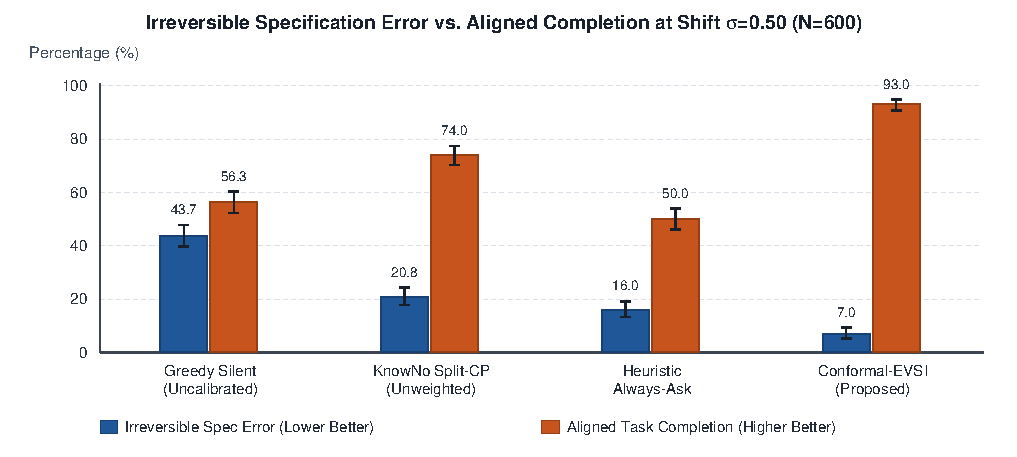
\includegraphics[width=0.88\textwidth]{figures/fig1_benchmark.pdf}
\caption{Comparison of Irreversible Specification Error Rate (lower is better) and Aligned Task Completion Rate (higher is better) on the paired test split at preference ambiguity and covariate shift $\sigma=0.50$ ($N_{\mathrm{cal}}=500,\allowbreak N_{\mathrm{test}}=600$ trajectories per architecture; error bars indicate asymmetric 95\% Wilson confidence intervals).}
\label{fig:benchmark}
\end{figure}

\begin{figure}[ht]
\centering
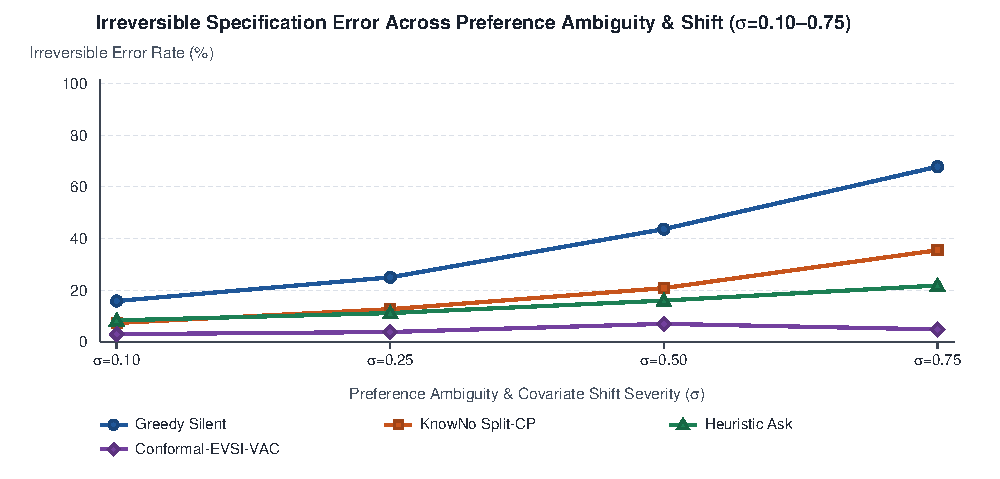
\includegraphics[width=0.86\textwidth]{figures/fig2_ablation.pdf}
\caption{Scaling of Irreversible Specification Error Rate across preference-ambiguity and covariate-shift severities $\sigma \in \{0.10,\allowbreak 0.25,\allowbreak 0.50,\allowbreak 0.75\}$ ($N_{\mathrm{test}}=600$ per cell). Unweighted KnowNo degrades under test-time shift as its static calibration quantile loses coverage, whereas Conformal-EVSI-VAC adapts set cardinality via observable sketch importance weights.}
\label{fig:ablation}
\end{figure}

% ===============================================================
\section{Adversarial failure modes, strategic abstention, and operational trade-offs}\label{sec:counter}

Deploying conformal deferral gates in personal agents confronts four substantive counter-arguments and failure modes documented in recent literature:

\begin{enumerate}
  \item \textbf{Reward hacking via strategic abstention (``Better Call Reward'', \citet{sahoo2026bettercall}).} If an agent's reinforcement learning objective directly rewards abstaining or deferring whenever uncertainty is high, policy optimization can game the deferral boundary itself. \citet{sahoo2026bettercall} demonstrate that optimizing legal and reasoning models with naive abstention rewards induces strategic non-commitment (the ``Saul Goodman effect''), where the model hedges and abstains on solvable tasks to collect safe abstention payouts. Consequently, Burden-of-Doubt Inversion must be enforced as a post-hoc runtime wrapper (\ref{eq:sketched_cp}) decoupled from policy training weights.
  \item \textbf{Shared constraint attribution and cyclic framing (\citet{cao2026lira, vaccaro2024combinations}).} When an agent queries local episodic memory ($q_{\mathrm{mem}}$) to filter candidate actions before presenting a Verifiable Action Card, the agent's retrieval framing influences the human's final selection. \citet{cao2026lira} show that learning responsibility allocation across shared human--AI constraints is non-trivial when errors arise from joint sequential decisions: if a stale memory trace ($\delta_{\mathrm{mem}}$) eliminates $a_t^*$ prior to human escalation, the user cannot recover the omitted option unless the VAC includes an explicit ``none of the above / edit raw parameters'' escape hatch.
  \item \textbf{Hardware friction of Inalienable Human-in-the-Loop (\citet{breckenridge2026ihitl}).} While boundary-rendered Verifiable Action Cards \citep{zhao2026clawguard} prevent prompt-level spoofing, \citet{breckenridge2026ihitl} prove that if host malware compromises the operating system display server, software confirmation dialogs can still be altered. Achieving full I-HITL security requires a physically separate secondary confirmation device (e.g., a mobile passkey push or smartwatch prompt), which increases interaction latency $c_{\mathrm{ask}}$.
  \item \textbf{Supervisory skill atrophy under automation (\citet{bainbridge1983ironies, eliav2026divergence, lee2025critical}).} Even when Conformal-EVSI-VAC reduces human queries to $0.20$ per task, \citet{bainbridge1983ironies} and \citet{lee2025critical} warn that automating the routine $80\%$ of unambiguous or memory-resolved tool executions gradually erodes the human operator's domain familiarity, potentially increasing $\delta_{\mathrm{VAC}}$ on complex edge-case escalations over multi-month horizons.
\end{enumerate}

% ===============================================================
\section{Limitations}\label{sec:limits}

\begin{itemize}
  \item \textbf{Synthetic logit benchmark versus live LLM evaluation on $\tau$-bench.} While \texttt{experiment.\linebreak[0]py} executes genuine split-conformal quantile calibration ($N_{\mathrm{cal}}=500$) and EVSI belief updating over $K=6$ structured candidate actions, the candidate logit distributions and shift norms are generated synthetically (Table~\ref{tab:provenance}). Validating Conformal-EVSI-VAC on live frontier and open-weight LLMs across full multi-turn $\tau$-bench retail and airline environments \citep{yao2024taubench} is the primary target of Falsification Protocol~P2.
  \item \textbf{Approximate coverage under estimated sketch weights ($\Delta_{\mathrm{sk}}$).} Because importance weights $\hat{w}(x)$ are computed from an estimated covariate sketch rather than the true unknown test density ratio, finite-sample conformal coverage under shift is approximate ($94.00\%$ [$91.81, 95.63$] empirical vs.\ $96.63\%$ nominal at $\sigma=0.50$, corresponding to $\Delta_{\mathrm{sk}} \approx 2.63\%$).
  \item \textbf{Discrete candidate enumeration.} Evaluating Equation~\eqref{eq:sketched_cp} requires a finite candidate set $\mathcal{A}_t$ of structured tool parameter tuples (obtained via diverse beam sampling or schema enumeration \citep{ren2023knowno, kuhn2023clam}), which adds sampling overhead when applied to free-text arguments.
\end{itemize}

% ===============================================================
\section{Pre-registerable falsification protocol}\label{sec:protocol}

Table~\ref{tab:protocol} defines six pre-registerable empirical tests that would falsify the coverage, error reduction, or query efficiency claims of the Conformal-EVSI-VAC gate.

\begin{table}[ht]
\centering
\small
\caption{Six pre-registerable falsification protocols for the Conformal-EVSI-VAC Burden-of-Doubt Inversion gate.}
\label{tab:protocol}
\begin{tabularx}{\textwidth}{@{}P{2.3cm}YYY@{}}
\toprule
Protocol & Hypothesis & Design and primary metrics & Falsified if \\
\midrule
P1. Post-hoc calibration under strategic inflation & Beta-Bernoulli calibration neutralizes ``Confidence Game'' inflation on tool candidates \citep{arghal2026confidence} & Evaluate 4 open/frontier models on 400 underspecified tool tasks under delegation-competing system prompts & Expected Calibration Error (ECE) after BBC exceeds $0.06$ or false singleton execution on ambiguous prompts exceeds $10.0\%$\\
P2. Live $\tau$-bench shifted coverage (Eq.~\ref{eq:sketched_cp}) & Sketched split-CP maintains $\ge 90\%$ empirical coverage under domain shift on live $\tau$-bench tasks \citep{yao2024taubench, ren2023knowno} & Calibrate on $N_{\mathrm{cal}}=500$ $\tau$-bench retail episodes and evaluate on $N_{\mathrm{test}}=500$ shifted airline/finance episodes with underspecified instructions & Empirical coverage $\Pr[a_t^* \allowbreak \in \hat{\mathcal{C}}(x_t)]$ drops below $90.0\%$ ($\Delta_{\mathrm{sk}} > 6.5\%$) or mean set size exceeds $3.0$\\
P3. EVSI query reduction vs.\ KnowNo & Two-tier EVSI local memory routing cuts human queries by $\ge 50\%$ vs.\ unweighted KnowNo \citep{ren2023knowno, zhang2024clarify} & Replay 600 longitudinal personal-assistant tasks with episodic user preference logs ($p_{\mathrm{mem}} \approx 0.65$) & Mean human queries per task exceeds $0.25$ or irreversible error increases by $>1.5$ percentage points vs.\ always-ask\\
P4. Out-of-band VAC spoofing resistance & Boundary-rendered Verifiable Action Cards block $100\%$ of prompt-level parameter substitutions \citep{breckenridge2026ihitl, zhao2026clawguard} & Red-team 300 compromised harness episodes attempting to swap tool AST parameters between prompt display and execution & Any mismatch ($>0.0\%$) between user-approved VAC parameters and executed tool AST is admitted\\
P5. Non-collapsing utility on unambiguous tasks & Post-hoc conformal gating avoids strategic abstention collapse on fully specified prompts \citep{sahoo2026bettercall} & Evaluate task completion on 400 fully specified, unambiguous $\tau$-bench instructions with Conformal-EVSI-VAC enabled & False deferral or persistent halt rate on unambiguous instructions exceeds $5.0\%$\\
P6. Break-even halt transition at $c_{\mathrm{ask}}^*$ & When $c_{\mathrm{ask}} > 0.40$, Tier~3 diverts unresolved ambiguities to safe halts rather than silent errors & Sweep clarification cost/latency constraints across $c_{\mathrm{ask}} \allowbreak \in [0.02,\allowbreak 0.65]$ on 600 ambiguous episodes & Irreversible specification error rises above $9.0\%$ when human clarification is suppressed at high $c_{\mathrm{ask}}$\\
\bottomrule\end{tabularx}
\end{table}

% ===============================================================
\section{Conclusion}\label{sec:conclusion}

Safe personal agency requires inverting the default burden of specification: when a user's instruction is underspecified over irreversible tool parameters, the runtime kernel must bound uncertainty and defer rather than guess silently, while respecting the cognitive limits of human attention. Extending split-conformal uncertainty alignment (KnowNo \citep{ren2023knowno}) and selective clarification (CLAM \citep{kuhn2023clam}, \citet{zhang2024clarify}), Conformal-EVSI-VAC combines Beta-Bernoulli epistemic calibration, covariate-sketched split-conformal prediction at capped quantile level $\tilde{q}(\alpha,\allowbreak \iota(f))$ with $+\infty$ quantile deferral under extreme shift, two-tier EVSI local memory pre-resolution, and out-of-band Verifiable Action Cards \citep{breckenridge2026ihitl}. Across 12{,}000 paired test trajectories (and 2{,}000 calibration episodes), Conformal-EVSI-VAC preserves $94.00\%$ [$91.81, 95.63$] empirical coverage under $\sigma=0.50$ covariate shift (where unweighted KnowNo drops to $84.50\%$ [$81.39, 87.18$]), reduces irreversible specification errors from $43.67\%$ [$39.75, 47.66$] (greedy) and $20.83\%$ [$17.77, 24.26$] (KnowNo) to $7.00\%$ [$5.22, 9.33$], and achieves $93.00\%$ [$90.67, 94.78$] aligned completion at $0.20$ human queries per task.

\section*{Use of AI tools}
Large language models were used to assist in drafting prose, formatting \LaTeX{} tables and TikZ diagrams, and implementing the standalone Python simulation script (\texttt{experiment.\linebreak[0]py}). Cited references were assembled from foundational computer-science literature and 2024--2026 research publications and checked against primary metadata records; simulation outputs, confidence intervals, and \LaTeX{} source packaging were verified using automated static consistency checks (\texttt{validate\_\linebreak[0]and\_\linebreak[0]package.\linebreak[0]py}).

\bibliographystyle{plainnat}
\bibliography{references}

\end{document}
